	\let\cleardoublepage\clearpage

\begin{spacing}{0.85}
	\sf
	\begin{center}
		\begin{minipage}{0.3\textwidth}
			\begin{center}
				\qquad {\fontfamily{pzc}\selectfont%
					République de Côte d'Ivoire\\
					\qquad  Union - Discipline - Travail
				}
			\end{center}
		\end{minipage}
	\end{center}
	
	\begin{minipage}{1\textwidth}
		\begin{minipage}{0.3\textwidth}
			\centering
			\begin{center}
				\begin{flushleft} 
				\end{flushleft}
			\end{center}
\includegraphics[width=5cm]{UNA}
			\DeclareGraphicsExtensions{.png,.jpg}
		\end{minipage}
		\hfill
		\begin{minipage}{0.3\textwidth}
			\begin{center}
				{\fontfamily{pzc}\selectfont%
					Ministère de l'enseignement Supérieur\\
					et de la Recherche Scientifique
				}
			\end{center}
		\end{minipage}
		\hfill
		\begin{minipage}{0.3\textwidth}
			\centering
			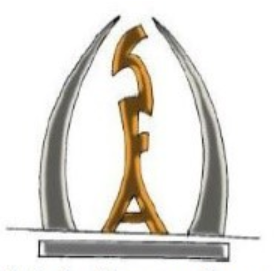
\includegraphics[width=4cm]{SFA.PNG}
			\DeclareGraphicsExtensions{.png,.jpg}
			{\fontfamily{pzc}\selectfont%
				Unité de Formation et de Recherche\\ 
				Sciences Fondamentales et Appliquées
			}
		\end{minipage}
	\end{minipage}
	
	\rule{1\textwidth}{4 pt}
	
	\begin{minipage}{1\textwidth}
		\begin{minipage}{0.4\textwidth}
			\begin{center}
				\rule{0.005cm}{4 pt}\shadowbox{N° d'ordre : LMI/MF/\ldots/2023 }
				\usefont{T1}{cmr}{m}{n}
			\end{center}
		\end{minipage}
		\hfill
		\begin{minipage}{0.4\textwidth}
			\begin{center}
				{\fontfamily{pzc}\selectfont%
					Année Académique : 2022-2023
				}
			\end{center}
		\end{minipage}\\
	\end{minipage}
	
	\begin{minipage}{1\textwidth}
		\begin{center}
			\textbf{MEMOIRE DE MASTER}
			\\
		\end{center}
		\begin{center}
			\textbf{MENTION}: MATHEMATIQUES\\
		\end{center}
		
		\begin{center}
			\textbf{OPTION}: OPTIMISATION, E.D.P ET ANALYSE NUMERIQUE\\
		\end{center}
		
		\begin{center}
			\textbf{SPECIALITE}: ANALYSE NUMERIQUE\\
		\end{center}
		\begin{center}
			PRESENTE PAR\\
		\end{center}
		\begin{center}
			\textbf{ASSOVIE BOKA GEDEON RUBEN}
			\\
		\end{center}
	\end{minipage}
	
	\begin{center}
		\underline{\textbf{THEME}}:
		\\
	\end{center}
	{\centering \qquad \setlength{\fboxsep}{1mm}
		\setlength{\fboxrule}{1mm}
		\fbox{\Ovalbox{\parbox{16cm}{\textbf{\color{purple} \begin{center}
							\begin{Large} APPROXIMATION NUMÉRIQUE DU TEMPS D'EXTINCTION POUR UNE ÉQUATION DE REACTION-DIFFUSION SOUMISE A DES CONDITIONS AUX LIMITES NON LINÉAIRES\\
		\end{Large}\end{center}}}}}\par}
	
	\begin{center}
		\begin{tabular}{ll}
			\textbf{DIRECTEUR de Mémoire}:  &  \textbf{YORO Gozo}, Maître de Conférences \\
			\\
			\textbf{ENCADRANT Scientifique}: &  \textbf{ \textbf{N'GUESSAN Koffi}}, Maître de Conférences
		\end{tabular}
	\end{center}
	\begin{center}
		Soutenu le \ldots 2023 devant le jury composé de
		\\
		
	\end{center}
	\begin{tabular}{lll}
		\hline \hline
		\emph{\textbf{Président}:}  DIAGANA Youssouf M. & Professeur Titulaire & \textbf{U}niversité \textbf{N}ANGUI \textbf{A}BROGOUA.\\
		\\
		\emph{\textbf{Membres}:}    nom et prénoms & Titre & \textbf{U}niversité \textbf{N}ANGUI \textbf{A}BROGOUA.\\
		\\
		\qquad \qquad \quad  nom et prénoms & Titre & \textbf{U}niversité \textbf{N}ANGUI \textbf{A}BROGOUA.\\
		\\
		\qquad \qquad  \quad    nom et prénoms & Titre & \textbf{U}niversité \textbf{A}LASSANE \textbf{O}UATTARA.\\
		\hline \hline
	\end{tabular}
\end{spacing}

\frontmatter
\tableofcontents